\documentclass[12pt, oneside]{article}
\usepackage[letterpaper, margin=1in, headsep=0.5in]{geometry}
\usepackage[english]{babel}
\usepackage[utf8]{inputenc}
\usepackage{amsmath}
\usepackage{amsfonts}
\usepackage{amssymb}
\usepackage{tikz}

\usepackage{fancyhdr}
\pagestyle{fancy}
\fancyhf{}
\rhead{\thepage \\Name: \hspace{1.5in}.\\}
\lhead{BECA / Dr. Huson / 11.2 Algebra 2\\* 14 May 2018 \\*\textbf{Test corrections: Exponential \& polynomial functions
}}

\renewcommand{\headrulewidth}{0pt}

\begin{document}

\subsection*{Do all problems. The numbers have changed.}
\vspace{1cm}

\begin{enumerate}

\item The expression $(x + a)(x + b)$ can not be written as
\begin{enumerate}
    \item $a(x + b)+ b(x + b)$
    \item $x^2 + ax + bx + ab$ 
    \item  $x^2 + (a + b)x + ab$  
    \item $x(x + a)+ b(x + a)$
\end{enumerate}

\item 
\begin{enumerate}
    \item What is the quotient and the remainder when $f(x)=3x^3+9x^2+8x-5$ is divided by $x+2$?\\*[5in]
    \item Given your answer to part (a), what is the value of $f(-2)$?
\end{enumerate}


\newpage
\item The expression $(x + a)(x - b)$ can not be written as
\begin{enumerate}
    \item $x(x + a)- b(x + a)$
    \item $x^2 + ax - bx - ab$ 
    \item  $x^2 + (a - b)x + ab$  
    \item $x(x - b)+ a(x - b)$
\end{enumerate}

\item A manufacturing company has developed a cost model, $C(x)=0.15x^3+0.01x^2+2x+120$, where $x$ is the number of items sold, in thousands. The sales price can be modeled by $S(x)=30-0.01x$. Therefore, revenue is modeled by $R(x)=x \cdot S(x)$.\\*[5pt]
The company’s profit, $P(x)=R(x)-C(x)$, could be modeled by what polynomial?  %Alg2 Regents Jun2017 multiple choice

\newpage

\item A bank account earns interest at a continuous interest rate of 3.925\% per year. The initial deposit is \$175. Which function models the value of the balance?
\begin{enumerate}
    \item $P(t)=175 \cdot 1.04^{t}$
    \item $P(t)=175 (1+0.03925)^{t}$
    \item $P(t)=175 \cdot 1.03925^{t}$
    \item $P(t)=175 \cdot e^{0.04t}$
\end{enumerate}

\item Carlos puts \$10,000 into an investment account with interest compounded continuously. If the annual interest rate is 3.75\% what is the balance after 4 years?\\[80pt]


\item Algebraically determine the values of $h$ and $k$ to correctly complete the identity stated below.
\[3x^3-5x^2+5=(x-2)(3x^2+hx+2)+k\] \\[2in] %Alg2 Regents Jan 2017


\item Simplify the expression $\sqrt{x^6 y^3}$.\\*[50pt]

\item Write $\sqrt[3]{a^5} \div a^{\frac{2}{3}}$ as an expression with positive, integer exponents.\\*[40pt]

\newpage

\item What is the expression $2i^3(-2i+5)$ is equivalent to? Express your answer in the form $a+bi$, where $a, b \in \mathbb{R}$.\\*[80pt]  %Alg2 Regents Jun2017 multiple choice

\item Simplify the expression $(1x - 3i)^2$, where $i$ is the imaginary unit. Express your answer in the form $a+bi$, where $a, b \in \mathbb{R}$.\\[80pt] %Alg2 Regents Aug2017

\item The function $p(t)=110e^{0.0325t}$ models the population of a city, in millions, $t$ years after 2010.
\begin{enumerate}
    \item Initially, as of 2010, what is the population in millions?\\[40pt]
    \item What is the annual continuous rate, expressed as in percent, that the population increases?\\[40pt]
    \item Find the population in 2015, rounded to the nearest million.\\[80pt]
    \item In what year will the population be approximately 138 million?
\end{enumerate}

\newpage

\item On the axes below, sketch a possible function $p(x) = (x  -a)(x - b)(x + c)$, where $a$, $b$, and $c$ are positive, $a  >b$, and $p(x)$ has a positive $y$-intercept of $d$. Label all intercepts. 
\begin{center}
    \begin{tikzpicture}[scale=2.54/4]
    \draw[thick,<->] (-7.5,0) -- (7.5,0) node[anchor=north west] {\textbf{x}};
    \draw[thick,<->] (0,-7.5) -- (0,7.5) node[anchor=south east] {\textbf{y}};
    \end{tikzpicture}
\end{center} %Alg2 Regents Aug2017

\item If $p(x)=2x^3-3x+5$, what is the remainder of $p(x) \div (x-5)$?%\\[5in] %Alg2 Regents Jan2018 multiple choice

\newpage

\item Graph $y=350(.75)^{0.8x}-50$ on the set of axes below.
\begin{center}
    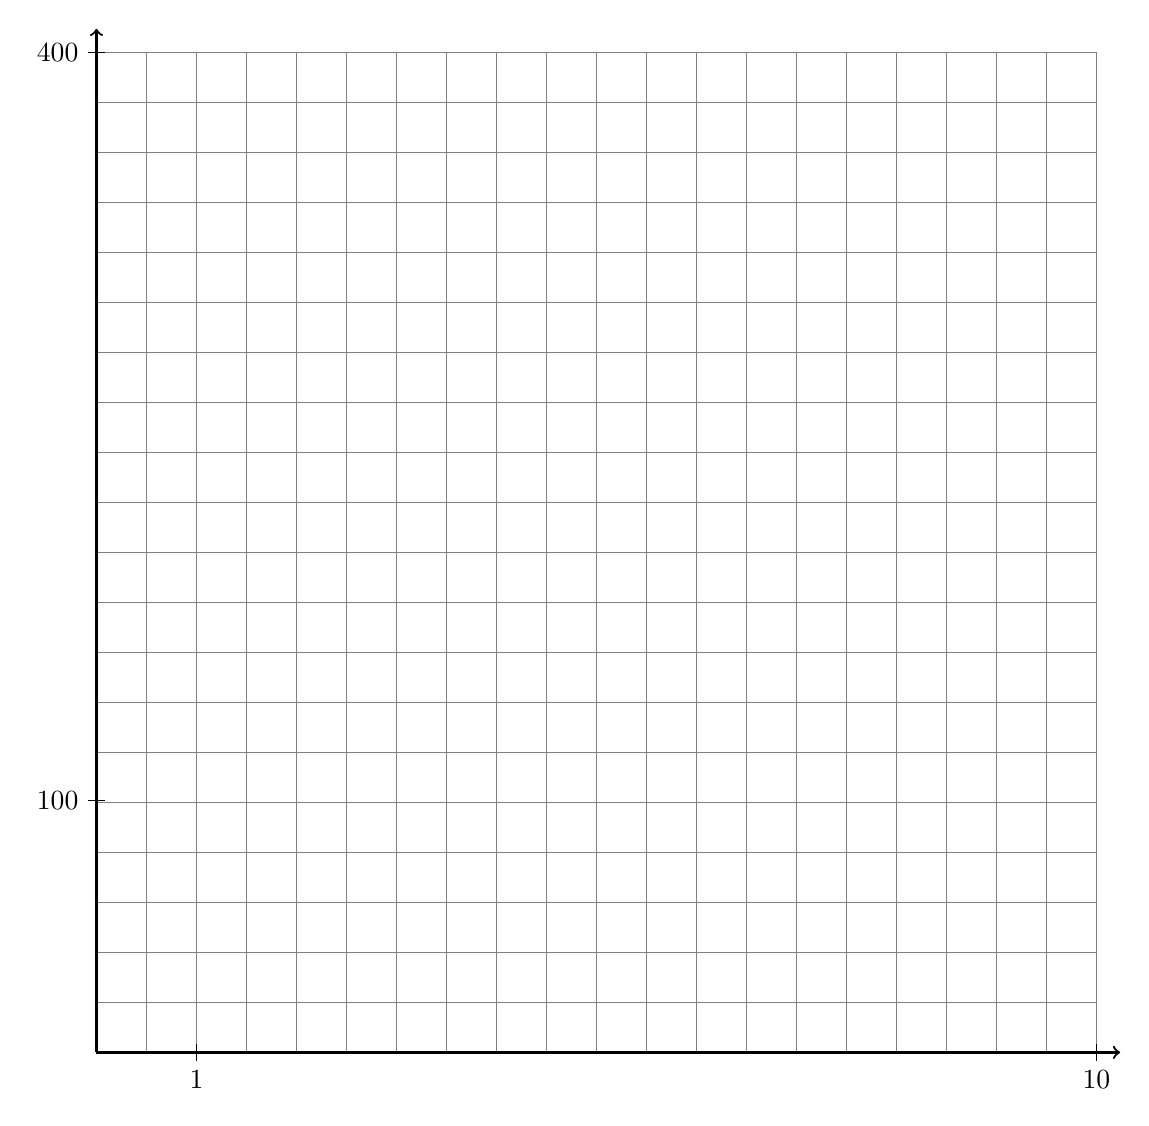
\begin{tikzpicture}
    \draw[step=0.25in,gray,very thin] (0,0) grid (12.7,12.7);
    \draw[thick,->] (0,0) -- (13,0); node[anchor=north west] {x};
    \draw[thick,->] (0,0) -- (0,13); node[anchor=south east] {y};
    \foreach \x in {1.27} \draw (\x cm,3pt) -- (\x cm,-3pt) node[anchor=north] {$1$};
    \foreach \x in {12.7} \draw (\x cm,3pt) -- (\x cm,-3pt) node[anchor=north] {10};
    \foreach \y in {3.2} \draw (3pt,\y cm) -- (-3pt,\y cm) node[anchor=east] {100};
    \foreach \y in {12.7} \draw (3pt,\y cm) -- (-3pt,\y cm) node[anchor=east] {400};
    \end{tikzpicture}
\end{center} %Alg2 Regents Jun2017

\item Explain how $\displaystyle (-27)^\frac{4}{3}$ can be evaluated using properties of rational exponents to result in an integer answer.

\end{enumerate}
\end{document}